\documentclass[MASTER.tex]{subfiles}
\begin{document}
%================================================================== %
\begin{frame}[fragile]
	\frametitle{Poisson Regression :  Crabs Example}
	\textbf{The crabs data set}
	The crabs data set is derived from Agresti \textit{(2007, Table 3.2, pp.76-77)}. It gives 4 variables for each of 173 female horseshoe crabs.
	\begin{itemize}
		\item \textbf{Satellites}
		number of male partners in addition to the female's primary partner
		
		\item \textbf{Width}
		width of the female in centimeters
		
		\item \textbf{Dark}
		a binary factor indicating whether the female has dark coloring (yes or no)
		
		\item \textbf{GoodSpine}
		a binary factor indicating whether the female has good spine condition (yes or no)
	\end{itemize}
\end{frame}
%================================================================== %
\begin{frame}[fragile]
	\frametitle{Poisson Regression :  Crabs Example}
	\begin{framed}
		\begin{verbatim}
		require(glm2)
		data(crabs)
		head(crabs)
		summary(crabs[,1:4])
		\end{verbatim}
		\end{framed}
	\end{frame}
	%================================================================== %
	\begin{frame}[fragile]
		\frametitle{Poisson Regression :  Crabs Example}
		\begin{verbatim}
		> head(crabs)
		Satellites Width Dark GoodSpine Rep1 Rep2
		1          8  28.3   no        no    2    2
		2          0  22.5  yes        no    4    5
		3          9  26.0   no       yes    5    6
		4          0  24.8  yes        no    6    6
		5          4  26.0  yes        no    6    8
		....
		\end{verbatim}
	\end{frame}
	%================================================================== %
	\begin{frame}[fragile]
		\frametitle{Poisson Regression :  Crabs Example}
		\begin{verbatim}
		> summary(crabs[,1:4])
		Satellites         Width       Dark     GoodSpine
		Min.   : 0.000   Min.   :21.0   no :107   no :121  
		1st Qu.: 0.000   1st Qu.:24.9   yes: 66   yes: 52  
		Median : 2.000   Median :26.1                      
		Mean   : 2.919   Mean   :26.3                      
		3rd Qu.: 5.000   3rd Qu.:27.7                      
		Max.   :15.000   Max.   :33.5                
		
		\end{verbatim}
	\end{frame}
	%================================================================== %
	\begin{frame}[fragile]
		\frametitle{Poisson Regression :  Crabs Example}
		Fit a Poisson regression model with the number of Satellites as the outcome and the width of the female as the covariate. What is the multiplicative change in the expected number of crabs for each additional centimeter of width?
		\begin{framed}
			\begin{verbatim}
			crabs.pois <- glm2(Satellites ~ Width, 
			data=crabs, family="poisson")
			summary(crabs.pois)
			exp(0.164)
			\end{verbatim}
		\end{framed}
		
	\end{frame}
	%================================================================== %
	\begin{frame}[fragile]
		\frametitle{Poisson Regression :  Crabs Example}
		\begin{verbatim}
		> summary(crabs.pois)
		
		Call:
		glm2(formula = Satellites ~ Width, 
		family = "poisson", data = crabs)
		
		...... 
		......
		Coefficients:
		Estimate Std. Error z value Pr(>|z|)    
		(Intercept) -3.30476    0.54224  -6.095  1.1e-09 ***
		Width        0.16405    0.01997   8.216  < 2e-16 ***
		---
		...... 
		\end{verbatim}
	
\end{frame}
%================================================================== %
\begin{frame}[fragile]
	\frametitle{Poisson Regression :  Crabs Example}
	\begin{figure}[h!]
		\centering
		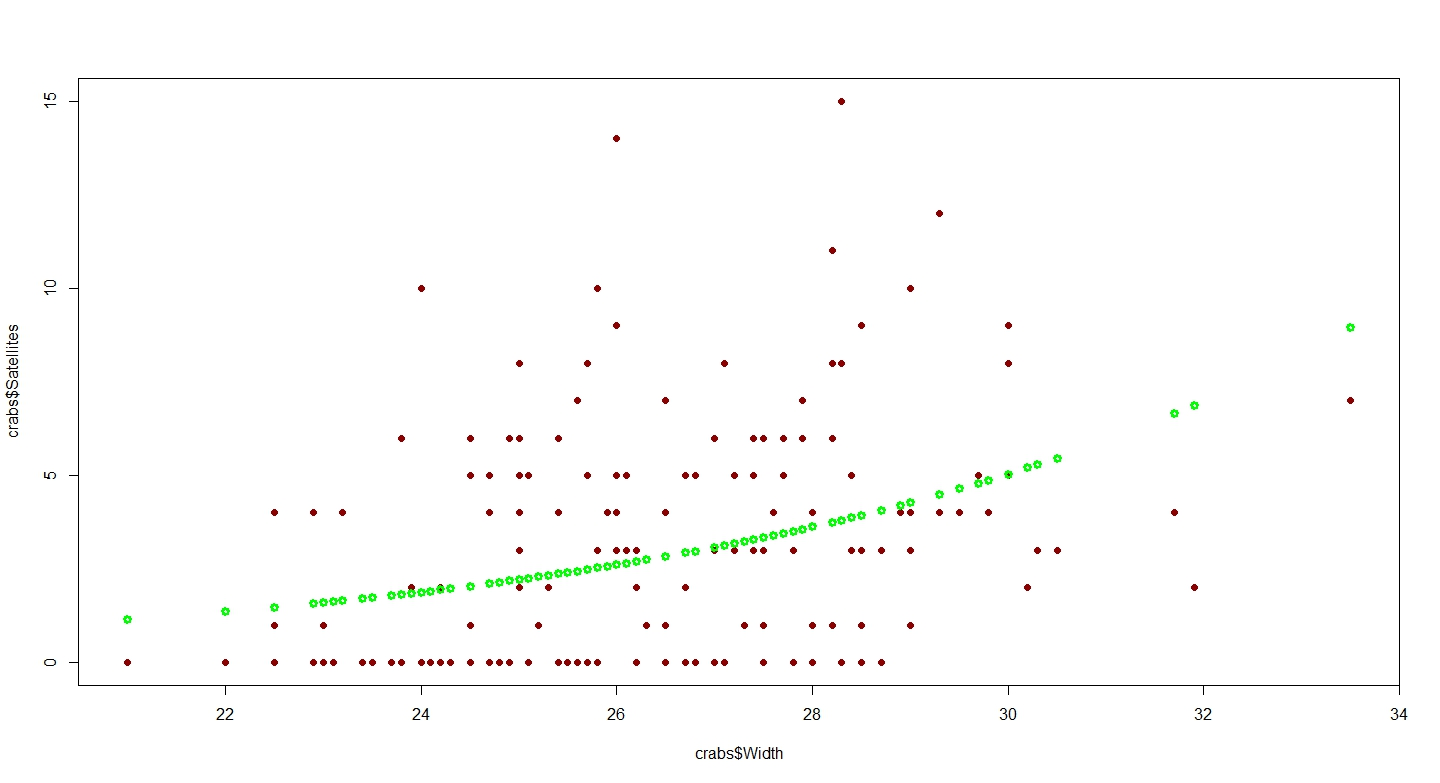
\includegraphics[width=1.05\linewidth]{./DAquiz5Q3c}
		%\caption{}
		%\label{fig:DAquiz5Q3c}
	\end{figure}
\end{frame}
%================================================================== %
\begin{frame}[fragile]
	\frametitle{Poisson Regression :  Crabs Example}
	
	\begin{framed}
		\begin{verbatim}
		plot(crabs$Width, crabs$Satellites,
		pch=16, col="darkred")
		points(crabs$Width, crabs.pois$fitted.values, 
		col="green", lwd=3)
		\end{verbatim}
	\end{framed}
\end{frame}
\end{document}